\documentclass[a4paper, 12pt]{article}
\usepackage[margin = 1in]{geometry}
\usepackage{graphicx}
\usepackage{amsmath,amssymb}
\setlength{\parindent}{0em}
\usepackage{float}
\usepackage{parskip}
\usepackage[dvipsnames]{xcolor}
\usepackage{tikz}


\title{\bfseries Inequality, Household Behavior, \& the Macroeconomy: Assignment 2}
\author{Max Heinze\and Gustav Pirich \and Berk Uzunonat}
\date{September 12, 2023}


\begin{document}

\maketitle

\section*{Problem 1}

\subsection*{Task 1.1}

Figure \ref{fig:graph11} shows assets, income and consumption paths of the model with altered parameters. Since we allow assets to vary between $-6$ and 6, and neither of those values is ever reached during the model's lifetime, we can conclude that the \textbf{borrowing constraints} are not binding. The \textbf{consumption path} is entirely flat, meaning that the agent consumes the same in each period of their life. The \textbf{wealth (assets) path} starts at zero, as the agent is born with no wealth, becomes negative as the agent borrows in order to satisfy their consumption needs, becomes positive in time for retirement, and then goes back to zero because the agent cannot consume after their death. Where borrowing constraints are not binding, we would expect from \textbf{theory} that consumption over the agent's lifetime is entirely flat, which coincides with the model output.

\begin{figure}[H]
    \centering
    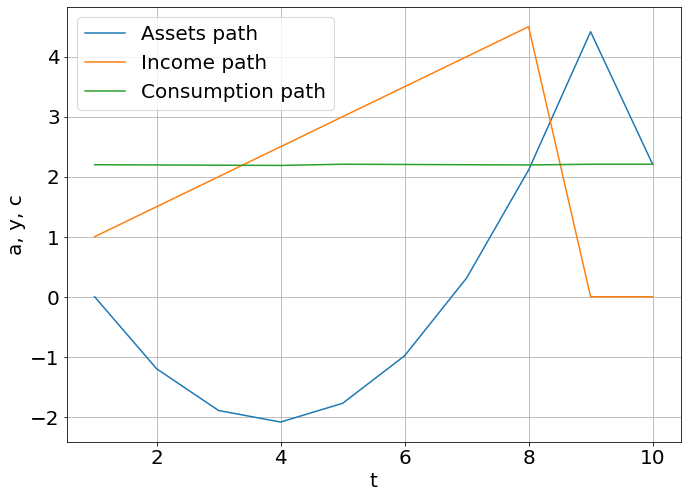
\includegraphics[width = 10cm]{task_1_1.png}
    \caption{Assets, income and consumption path for the model in question.}
    \label{fig:graph11}
\end{figure}

\subsection*{Task 1.2}

To derive the optimal consumption path, we need to solve the following maximization problem:

\[
    \underset{c_t,a_{t+1}}{\mathrm{max}}\sum^{10}_{t=0}\underbrace{\beta^t}_{=1}u(c_t) \qquad \mathrm{s.t.} \qquad a_{t+1}=\underbrace{(1+r)}_{=1}a_t+y_t-c_t
\]

We get the following Lagrangian and FOC:

\begin{align*}
    \mathcal{L} &= \sum^{10}_{t=0}u(c_t)+\lambda_t(a_t+y_t-c_t-a_{t+1})\\
    \\
    \frac{\partial\mathcal{L}}{\partial c_t} &= \frac{\partial u(c_t)}{\partial c_t} - \lambda_t\qquad \overset{!}{=} 0  \\
    \frac{\partial\mathcal{L}}{\partial a_{t+1}} &= -\lambda_t + \lambda_{t+1}\qquad \overset{!}{=} 0 
\end{align*}

Since 

\[
    \frac{\partial u(c_t)}{\partial c_t} = c_t^{-2},
\]

it follows that

\[
    c_t^{-2} = c_{t+1}^{-2},
\]

from which we get in turn

\[
    c_t = c_{t+1},
\]

meaning that consumption is constant and thus the sum over all lifetime consumption is just $t$ times that constant consumption of any period.

Since income is given as

\[
    y_t = 
    \begin{cases}
        1 + 0.5t & \text{for $t = 0,\dots, 7$}\\
        0 & \text{otherwise}
    \end{cases},
\]

the sum of all lifetime income equals 

\[
    \sum^{10}_{t=0}y_t = 22,
\]

which divided by 10 periods of consumption yields a level of consumption per period of 2.2, which corresponds to the level from the model output. There are slight differences between the model values and 2.2, which is due to the discrete, and therefore inexact, nature of the simulated model. The asset grid, through which the optimal level of savings is determined in the Python script does not allow to determine the optimal level of savings exactly. However, the solution is extremely close to the optimal outcome as can be seen on the graph. 

\begin{figure}[H]
    \centering
    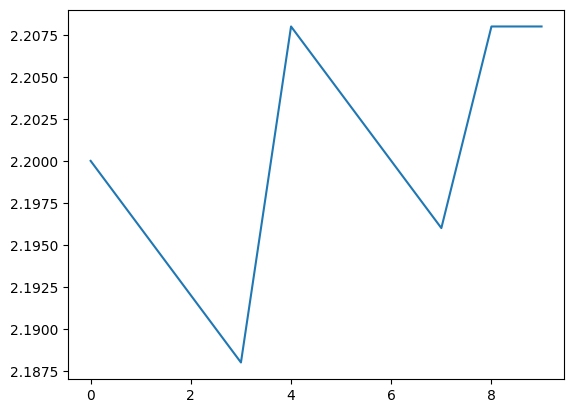
\includegraphics[width = 10cm]{task_1_2.png}
    \caption{The values of the consumption path in the simulated model are all very close to 2.2.}
    \label{fig:graph12}
\end{figure}

\subsection*{Task 1.3}

Consumption is equal in both scenarios since the interest rate is zero. In this case neither saving nor borrowing assets can changes the overall disposable income, which is solely determined by the income path. Under the non-binding borrowing constraint scenario, the agent is smoothing consumption by borrowing money in the first periods, yielding a flat consumption path. Due to the specification of the utility function with ($u_c > 0$ and $u_{cc} < 0$), a stable consumption path maximizes lifetime utility. Under the binding borrowing constraint scenario, the agent has a lower level of consumption in the first periods, and a slightly higher level in the later periods. However due to the specification of the utility function, this leads to an overall lower level of welfare.

\begin{table}[H]
\centering
\begin{tabular}{l|cc}
\multicolumn{1}{c|}{\textbf{$r = 0 $}} & \textbf{Borrowing constraint} & \textbf{No borrowing constraint} \\ \hline
\textbf{Consumption}                   & 22                            & 22                               \\
\textbf{Utility}                       & -4.9667                       & -4.5455                         
\end{tabular}
\caption{Utility and consumption for the case $r = 0$.}
\label{table:r0}
\end{table}

\begin{table}[H]
\centering
\begin{tabular}{l|cc}
\multicolumn{1}{c|}{\textbf{$r = 0.05 $}} & \multicolumn{1}{c}{\textbf{Borrowing constraint}} & \multicolumn{1}{c}{\textbf{No borrowing constraint}} \\ \hline
\textbf{Consumption}                      & 22.6208                                           & 21.9368                                              \\
\textbf{Utility}                          & -4.0851                                           & -3.6577                                             
\end{tabular}
\caption{Utility and consumption for the case $r \approx 0.05$.}
\label{table:r0005}
\end{table}

In the second case consumption is higher under the binding borrowing constraint. This is because of the interest rate, which affects the overall consumption over the lifetime in two ways. First, the interest rate increases the cost of borrowing. Secondly under the non-binding borrowing constraint scenario the agent is saving slightly more assets, which will yield a higher rate of return. Both effects lead to the observed pattern, that the binding borrowing constraint increases the overall level of consumption. However, since the agent prefers smooth consumption (To fulfill the Euler equation, $\beta*(1+r) < 1 $, it is optimal that agents consume slightly more today than tomorrow), the overall level of utility is higher under the non-binding borrowing constraint scenario as the agent can finance a higher level of consumption in the first periods. 

\subsection*{Task 1.4}

The lagrangian multiplier shows the marginal utility of relaxing the borrowing constraint by one unit. If mu ($\mu$) is positive, the constraint is binding. The graph shows the trajectory over the lifetime of the agent. In the first period relaxing the borrowing constraint would bring large utility gains to the consumer as her income is low and consumption is low. The marginal utility of increasing consumption by one unit would therefore bring large benefits. In the subsequent periods the benefit declines exponentially. In period 3 the marginal benefit of relaxing the resource constraint is extremely small as current disposable income is already relatively high. From period 4 onwards the constraint is not binding. 

\begin{figure}[H]
    \centering
    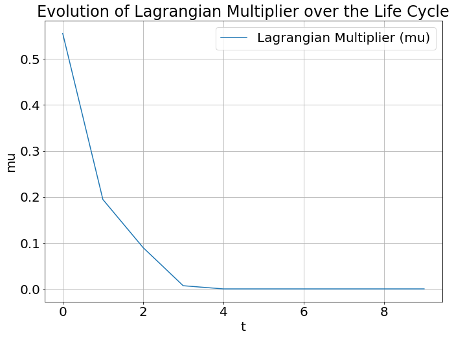
\includegraphics[width = 10cm]{task_1_4.png}
    \caption{The path of the Lagrangian multiplier over time, $\lambda_t$.}
    \label{fig:graph14}
\end{figure}

\subsection*{Task 1.5}

Comparing scenario A and B, we find that discounting the future leads to a declining optimal consumption path over the life cycle. From the Euler equation it can be seen that the agent must consume more in earlier periods. $U'(C_{t}) = 0.6*U'(C_{t+1})$ To fulfill Euler equation, the agent borrows heavily in the first four periods. In figure 4 it can be seen that the borrowing constraint becomes binding after four periods as assets reach the lowest level of -6. The interest rate is set to zero, which implies that the agent is not incurring costs for the high level of borrowing.

Comparing scenario B and C, we see that consumption tracks income growth over the first periods, as the borrowing constraint is binding. After seven periods the agent starts to save for retirement. Assets are increasing to finance the consumption over for the retirement period. Consumption declines after period six. The presence of discounting makes earlier consumption relatively more attractive than later consumption. Thus the optimal consumption path is declining over the lifetime of the consumer.   
This scenario appears to track the empirically observed consumption and income patterns. We see the inverted U- (or in this case rather V shaped) consumption path. The fact that consumers are relatively impatient necessitates a declining optimal consumption path, as earlier periods bring a higher level of utility than later periods. In period 6-8, when the agent starts to save for retirement, earnings exceed consumption. This can also be observed in the CES graphs. To summarize the graph reflects two distinctive empirical facts 1) the hump shaped consumption pattern, and 2) the drop of consumption with retirement. 

\begin{figure}[H]
    \centering
    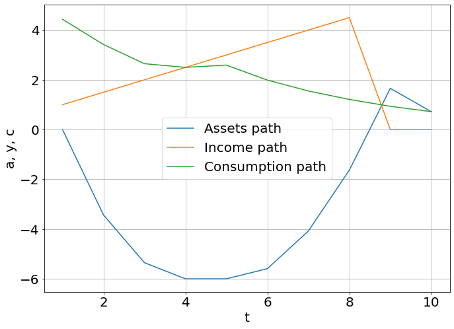
\includegraphics[width = 10cm]{task_1_5a.png}
    \caption{Scenario A: The model simulated with $beta = 0.6$ and $a_{\mathrm{min}} = -6$.}
    \label{fig:graph15a}
\end{figure}

\begin{figure}[H]
    \centering
    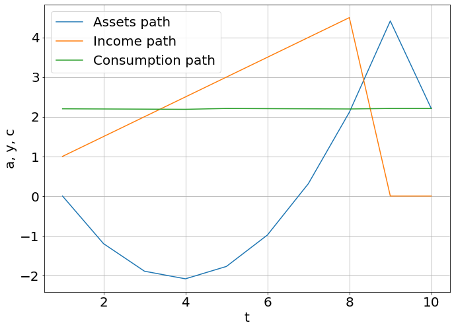
\includegraphics[width = 10cm]{task_1_5b.png}
    \caption{Scenario B: The model simulated with $beta = 1$ and $a_{\mathrm{min}} = -6$.}
    \label{fig:graph15b}
\end{figure}

\begin{figure}[H]
    \centering
    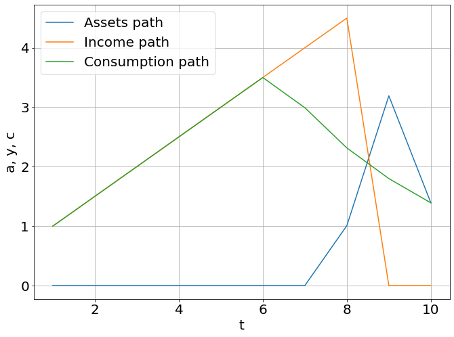
\includegraphics[width = 10cm]{task_1_5c.png}
    \caption{Scenario C: The model simulated with $beta = 0.6$ and $a_{\mathrm{min}} = 0$.}
    \label{fig:graph15c}
\end{figure}

\section*{Problem 2}

Zeldes (1989) tests the null hypothesis that households smooth consumption over their life cycle as predicted by the PIH against the alternative that agents are maximizing lifetime utility subject to a set of borrowing constraints. In contrast to preceding papers, he does not test the PIH against, either the alternative that the model does not fit the data or that consumers behave "Keynesian" (i.e. consumption equals a share of income).

All tests are based on the Euler equation, derived from the maximization of expected lifetime utility. The equation implies that the marginal utility from consuming one unit today should be equal to the discounted expected marginal utility from what the agent would have received if the unit was invested and consumed in the future period.

The \textbf{first test} is based on a regression of the growth of food consumption on a set of fixed effects, control variables and income. Zeldes (1989) splits the sample into two groups. The sample restriction is based on whether the borrowing constraint is likely to be binding (Group 1) or not (Group 2). If a household at any given time point belongs to group 1, the Lagrangian multiplier on the constraint is necessarily positive. Relaxing the constraint would therefore increase expected lifetime utility. Current disposable income should enter the equation negative and significantly as predicted by the borrowing constraint theory. Likewise if a household belongs to group 2 current disposable income should not have a significant impact on consumption growth. The split is based on the liquid financial assets, excluding housing assets to income ratio. Zeldes (1989) uses a sample split because it is not possible to derive a closed-from expression of the Lagrangian multiplier.

The first test shows that for group 1, current income reduces the growth of consumption statistically significantly, as predicted by the borrowing constraints theory. For group 2 income does not affect consumption growth significantly. The prediction of the Euler equation is thus violated for the borrowing constrained group 1, whilst in line for group 2. 

The \textbf{second test} is based on the one-sided inequality of the Euler equation. The Lagrangian multiplier $\lambda_{it}$ can only be strictly positive if it exists for group 1. This is because Zeldes (1989) tests the hypothesis that households in group 1 are borrowing, but not saving constraint. He tests the size and direction of the average Lagrangian multiplier for group 1 by constructing an estimate for the population level Lagrangian multiplier from group 2. He finds that there is a positive and statistically significant effect only at the $10\%$ level. Excess consumption growth due to the borrowing constraint for group 1 amounts to on average $1.7\%$. Thus the borrowing constraint theory is somewhat supported in this case but the evidence is not strong. 

The \textbf{third test} is based on whether the Lagrangian multiplier $\lambda_{it}$ is negatively related to current real disposable income $y_{it}$. The premise is that higher current income should lead to diminished utility from easing the borrowing constraints. Zeldes $(1989)$ uses $\hat{x}_{it+1}$, a consistent estimate of group 1's average excess growth in consumption due to borrowing constraint. He finds a negative, albeit not statistically significant relationship between income and excess consumption growth. However this regression estimates a total derivative. The results of the third test are theoretically and empirically not clear cut, since Zeldes (1998) fails to identify the partial derivative, with a ceteris paribus interpretation. Should an increase in current disposable income signal an even higher anticipated future income stream as well, the lagrangian multiplier on the borrowing constraint might even increase.

\section*{Problem 3}

Let there be two different groups of people in a society, those that go to college and those that do not. Assume that the income of both groups of people starts at zero, but that college-goers' income increases twice as fast. After $T_R$ periods, individuals retire, after which they earn a pension income in each period that is proportional to their income in the last period before retirement, that is, 

\[
    y_{T_R+1,j} = sy_{T_R,j},
\]

where $j \in \{0,1\}$ denotes the group (college-goers or non-college-goers) and $s$ the replacement rate of the pension system, which we assume identical over both $j$. Let us further say individuals die after $T$ periods. Plotting income over the lifetime then looks somewhat like this:

\begin{figure}[H]
    \centering
    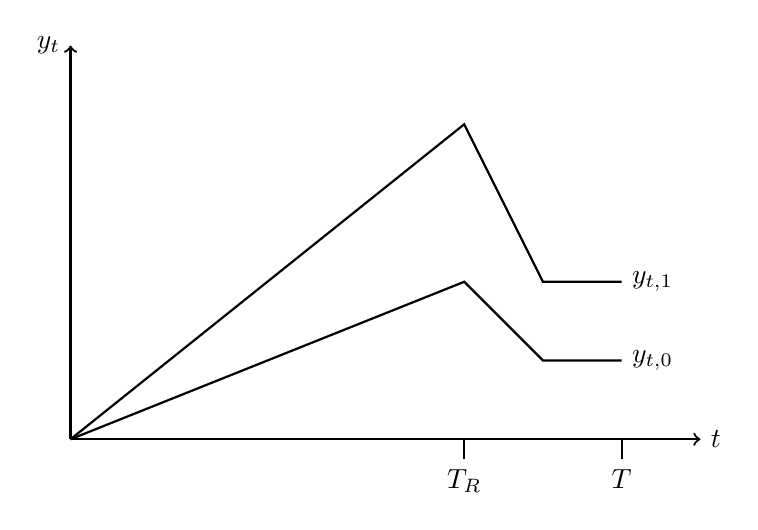
\begin{tikzpicture}[thick]
        \draw[->] (0,0) -- (8,0) node[right] {$t$};
        \draw[->] (0,0) -- (0,5) node[left] {$y_t$};
        \draw (0,0) -- (5,2) -- (6,1) -- (7,1) node[right] {$y_{t,0}$};
        \draw (0,0) -- (5,4) -- (6,2) -- (7,2) node[right] {$y_{t,1}$};
        \draw (5,0) -- (5,-0.25) node[below] {$T_R$};
        \draw (7,0) -- (7,-0.25) node[below] {$T$};
    \end{tikzpicture}
    \caption{Income paths for both groups with a replacement rate of 50 percent.}
    \label{fig:graph3a_1}
\end{figure}

More concisely and formally, let income be given by

\[
    y_{t,j} = 
    \begin{cases}
        g_j t  & \text{for $t \leq T_R$},\\
        sg_j T_R  & \text{otherwise},
    \end{cases}
\]

where $g_j$ is the amount by which a group's income grows in each period and $g_1 = 2g_0$. If we further assume that there is neither an interest rate nor do people discount, and that consumers' utility functions are concave, we can easily deduct that the optimal consumption path for any consumer is one that keeps consumption constant. Consumption per period is then given by

\[
    c_t = \overline{c} = T^{-1}\left(\frac{T_R(T_R+1)g_j}{2}+(T-T_R)T_Rsg_j\right),
\]

from which we can easily see that if income grows twice as quickly for college graduates, consumption is twice as high for them, i.e.

\[
    \overline{c}_{1} = 2\overline{c}_{0}.
\]

Plotting this, we get the following:

\begin{figure}[H]
    \centering
    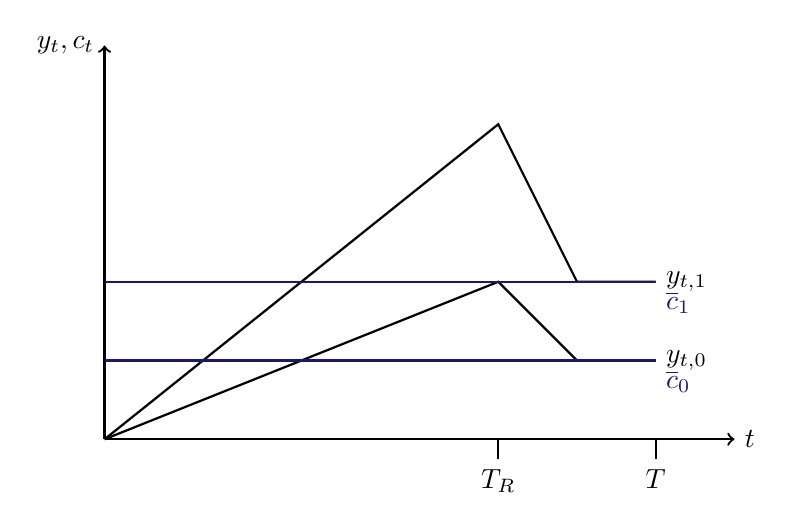
\begin{tikzpicture}[thick]
        \draw[->] (0,0) -- (8,0) node[right] {$t$};
        \draw[->] (0,0) -- (0,5) node[left] {$y_t,c_t$};
        \draw (0,0) -- (5,2) -- (6,1) -- (7,1) node[right] {$y_{t,0}$};
        \draw (0,0) -- (5,4) -- (6,2) -- (7,2) node[right] {$y_{t,1}$};
        \draw (5,0) -- (5,-0.25) node[below] {$T_R$};
        \draw (7,0) -- (7,-0.25) node[below] {$T$};
        \draw[MidnightBlue] (0,2) -- (7,2) node[below right] {$\overline{c}_1$};
        \draw[MidnightBlue] (0,1) -- (7,1) node[below right] {$\overline{c}_0$};
    \end{tikzpicture}
    \caption{Income and consumption paths for both groups with a replacement rate of 50 percent.}
    \label{fig:graph3a_2}
\end{figure}

Next up, savings. These are just given by the difference of income and consumption, as in

\[
    \Delta a_{t,j} = y_{t,j} - \overline{c}_{j}.
\]

Since at any point in time, both income and consumption of college-educated people are twice as high as that of non-college-goers, 

\[
    \Delta a_{t,1} = 2\Delta a_{t,0}.
\]

Adding this to the plot:

\begin{figure}[H]
    \centering
    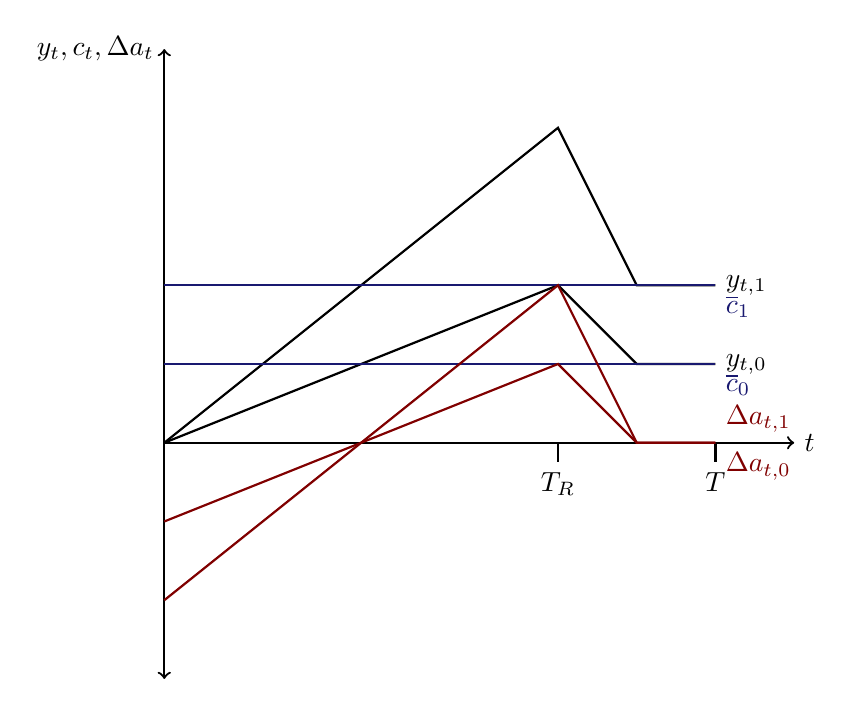
\begin{tikzpicture}[thick]
        \draw[->] (0,0) -- (8,0) node[right] {$t$};
        \draw[<->] (0,-3) -- (0,5) node[left] {$y_t,c_t,\Delta a_t$};
        \draw (0,0) -- (5,2) -- (6,1) -- (7,1) node[right] {$y_{t,0}$};
        \draw (0,0) -- (5,4) -- (6,2) -- (7,2) node[right] {$y_{t,1}$};
        \draw (5,0) -- (5,-0.25) node[below] {$T_R$};
        \draw (7,0) -- (7,-0.25) node[below] {$T$};
        \draw[MidnightBlue] (0,2) -- (7,2) node[below right] {$\overline{c}_1$};
        \draw[MidnightBlue] (0,1) -- (7,1) node[below right] {$\overline{c}_0$};
        \draw[Maroon] (0,-1) -- (5,1) -- (6,0) -- (7,0) node[below right] {$\Delta a_{t,0}$};
        \draw[Maroon] (0,-2) -- (5,2) -- (6,0) -- (7,0) node[above right] {$\Delta a_{t,1}$};
    \end{tikzpicture}
    \caption{Income, consumption, and savings paths for both groups with a replacement rate of 50 percent. Note that savings are plotted, not their cumulative sum.}
    \label{fig:graph3a_3}
\end{figure}

Now, what is inequality? Let us first assume something about the structure of the society before we talk about differences in its members. Say there is a number of members $N$, and a share of college-goers $\gamma$ that is constant in all age groups. An age group is, of course, just one possible value of $t$. Say further that individuals are evenly distributed between all possible age groups (we need them to be in different stages of their lives, otherwise all members of a group would be perfectly equal and all inequality would disappear if everybody was going to college). That is, in each and every age group, there is some number $NT^{-1}\gamma$ of people who went to college and $NT^{-1}(1-\gamma)$ who did not.

In the example used in the plot, all individuals are at all times either in debt or, at best, have no wealth. This is because the replacement rate is high enough for the constant consumption to be financed by pension income. It also makes for a more intuitive reasoning. Before we talk about inequality in more detail, let us first plot assets:

\begin{figure}[H]
    \centering
    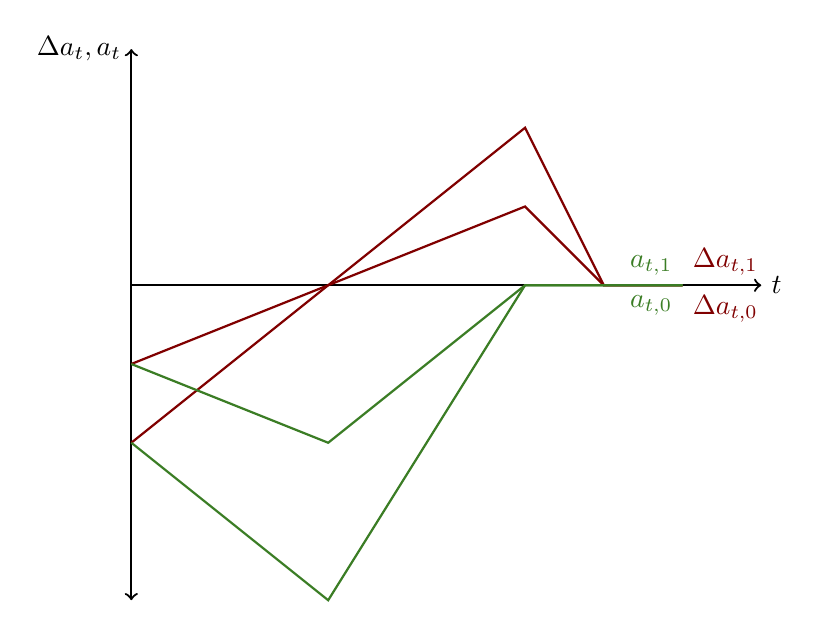
\begin{tikzpicture}[thick]
        \draw[->] (0,0) -- (8,0) node[right] {$t$};
        \draw[<->] (0,-4) -- (0,3) node[left] {$\Delta a_t, a_t$};
        \draw[Maroon] (0,-1) -- (5,1) -- (6,0) -- (7,0) node[below right] {$\Delta a_{t,0}$};
        \draw[Maroon] (0,-2) -- (5,2) -- (6,0) -- (7,0) node[above right] {$\Delta a_{t,1}$};
        \draw[OliveGreen] (0,-1) -- (2.5,-2) -- (5,0) -- (7,0) node[below left] {$a_{t,0}$};
        \draw[OliveGreen] (0,-2) -- (2.5,-4) -- (5,0) -- (7,0) node[above left] {$a_{t,1}$};
    \end{tikzpicture}
    \caption{Savings and asset paths for both groups with a replacement rate of 50 percent.}
    \label{fig:graph3a_4}
\end{figure}

Using a reasonable measure of inequality, such as the variance of all people's assets, an increase of $\gamma$ to 1 would \textbf{increase} the level of inequality, as there would be more people that are in very high debt as compared to the baseline scenario, where some people's debt is just half as high.

What about the replacement rate? Increasing it would yield higher consumption, but it would still need to be smoothed over the entire lifetime of individuals. Of course, individuals would in this adapted scenario still not save anything, but rather borrow first and repay their debt later, just in time for them to be debt-free upon dying. However, the amount they borrow has increased, as they consume more. Thus, by the argument presented above, a higher replacement rate would \textbf{increase} inequality.

We conclude that in the very narrow scenario we set ourselves, \textbf{inequality in a society with only college-goers, and in a society with a high pension replacement rate, will be higher, ceteris paribus}. The statement could therefore be regarded as \textbf{TRUE}.

\textbf{HOWEVER}, considering any other factor, such as how the pension system is financed, heterogeneous income within groups, possible borrowing constraints, etc., renders the question ambiguous and impossible to answer, which would yield the conclusion that the answer is in fact \textbf{UNCERTAIN}.


\end{document}
